\documentclass[uplatex, dvipdfmx, a4paper, report, papersize, 11pt]{jsbook}
\usepackage{bm}
\usepackage{amsmath}
\usepackage[dvipdfmx]{graphicx}
\usepackage{wrapfig}
\usepackage[hang, small, bf]{caption}
\usepackage[subrefformat=parens]{subcaption}
\usepackage{here}
\usepackage{comment}
\captionsetup{compatibility=false}

\bibliographystyle{junsrt}

\title{\fontsize{24.88pt}{0pt}\selectfont 卒業論文 \vspace{2cm}\\ 二色の光周波数コムによる\vspace{4mm}\\ レーザー冷却法の開拓 \vspace{3cm}\\ \fontsize{17.28pt}{0pt}\selectfont 指導教員\ \ \ \ \ 吉岡孝高\ \ 准教授 \vspace{4cm}\\ \fontsize{17.28pt}{0pt}\selectfont  平成31年2月提出 \vspace{2cm} \\ \fontsize{17.28pt}{0pt}\selectfont 東京大学工学部物理工学科 \vspace{3mm} \\ 03-170579\ \ \ 中西亮}
\date{}

\begin{document}
\begin{center}
  \Huge 卒業論文 \par
  \vspace{20mm}
  \Huge 二色の光周波数コムによる \par
  \vspace{4mm}
  \Huge レーザー冷却法の開拓 \par
  \vspace{30mm}
  \LARGE 指導教員\ \ \ \ \ 吉岡孝高\ \ 准教授\par
  \vspace{30mm}
  \LARGE 平成31年2月提出\par
  \vspace{15mm}
  \LARGE 東京大学工学部物理工学科 \par
  \vspace{10mm}
  \LARGE 03-170579\ \ \ 中西亮
  \vspace{10mm}
\end{center}
\thispagestyle{empty}
\clearpage
\addtocounter{page}{-2}
\newpage
\thispagestyle{empty}
 
\newpage

\setcounter{tocdepth}{2}
\tableofcontents

\newpage

\chapter{増幅実験}
\section{結論}

今回の実験では$766$ nm付近の波長では$35$ mW, $890$ nm付近の波長では$70$ mWのパワーを得た. 図\ref{rityounashi_level_diagram}のように、コムの中心周波数と、中間準位への共鳴周波数が一致するようなスペクトルを考えると、このパワーのときに近共鳴な中間準位への一光子励起効率は$3\times 10^2\ \mathrm{s^{-1}}$となる. このとき, 実験で得られたパワーでの二光子冷却の励起効率を見積もると$8.2\times10^3\ \mathrm{s^{-1}}$であることが分かり, 励起効率を二色のパワーによりプロットすると図\ref{result-colorplot}のようになる. \par
なお, 上記の見積もりはビームスポットの直径が$0.5$ mmとして計算を行ったが, 光の強度はビームスポットに反比例するために式(\ref{approx_ex-rate})のように強度の二乗に比例する二光子の励起効率は, ビームスポットの直径の四乗に反比例する. \par
$766$ nmのコムの増幅に用いたTAは今回の実験では$1600$ mAまでしか駆動させなかったが, 最大で$3500$ mAまで印加することができる. 同様に, $890$ nmのコムの増幅に用いたTAは今回の実験では$3$ Aまでしか駆動させなかったが, 最大で$4$ Aまで印加することができる. このため, 今回の実験系でもTAの印加電流を上げることでまだ増幅率の向上の余地はあると考えられる. \par

\begin{figure}[H]
  \centering
    \begin{tabular}{c}
      \begin{minipage}{1\hsize}
        \centering
          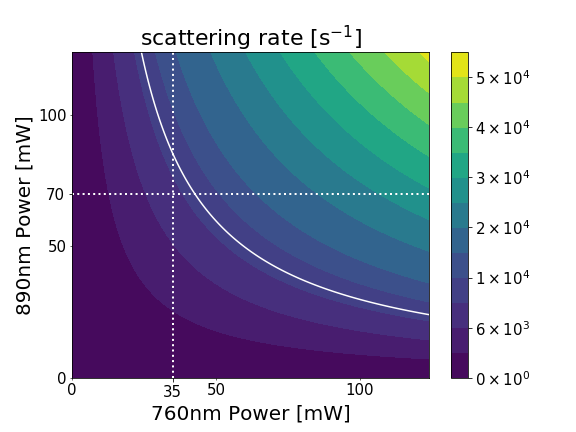
\includegraphics[keepaspectratio,  scale=0.5,  angle=0]
          {figures/chapter4/rityounashi_result.png}
          \caption{$6P_{\frac{1}{2}}$と最近接の一光子コムの歯の離調が$700$ MHzのときの二光子励起効率の二色のパワー依存性. 白点線の交点で示されている点が今回得られた二色のパワーの組み合わせである. この点では$8.2\times 10^3\ \mathrm{s^{-1}}$の励起効率が見積もられる。白実線で示されているのが$10000\ \mathrm{s^{-1}}$の励起効率の曲線である. ビームスポットの直径は$0.5$ mm, 繰り返し周波数は$1.6$ GHz, コムの周波数幅は$5$ THzである.}
          \label{result-colorplot}
      \end{minipage}
    \end{tabular}
\end{figure}

\bibliography{reference}
\end{document}
